%%
%% Automatically generated file from DocOnce source
%% (https://github.com/hplgit/doconce/)
%%
%%


%-------------------- begin preamble ----------------------

\documentclass[%
oneside,                 % oneside: electronic viewing, twoside: printing
final,                   % draft: marks overfull hboxes, figures with paths
10pt]{article}

\listfiles               %  print all files needed to compile this document

\usepackage{relsize,makeidx,color,setspace,amsmath,amsfonts,amssymb}
\usepackage[table]{xcolor}
\usepackage{bm,ltablex,microtype}

\usepackage[pdftex]{graphicx}

\usepackage[T1]{fontenc}
%\usepackage[latin1]{inputenc}
\usepackage{ucs}
\usepackage[utf8x]{inputenc}

\usepackage{lmodern}         % Latin Modern fonts derived from Computer Modern

% Hyperlinks in PDF:
\definecolor{linkcolor}{rgb}{0,0,0.4}
\usepackage{hyperref}
\hypersetup{
    breaklinks=true,
    colorlinks=true,
    linkcolor=linkcolor,
    urlcolor=linkcolor,
    citecolor=black,
    filecolor=black,
    %filecolor=blue,
    pdfmenubar=true,
    pdftoolbar=true,
    bookmarksdepth=3   % Uncomment (and tweak) for PDF bookmarks with more levels than the TOC
    }
%\hyperbaseurl{}   % hyperlinks are relative to this root

\setcounter{tocdepth}{2}  % levels in table of contents

% Tricks for having figures close to where they are defined:
% 1. define less restrictive rules for where to put figures
\setcounter{topnumber}{2}
\setcounter{bottomnumber}{2}
\setcounter{totalnumber}{4}
\renewcommand{\topfraction}{0.95}
\renewcommand{\bottomfraction}{0.95}
\renewcommand{\textfraction}{0}
\renewcommand{\floatpagefraction}{0.75}
% floatpagefraction must always be less than topfraction!
% 2. ensure all figures are flushed before next section
\usepackage[section]{placeins}
% 3. enable begin{figure}[H] (often leads to ugly pagebreaks)
%\usepackage{float}\restylefloat{figure}

% prevent orhpans and widows
\clubpenalty = 10000
\widowpenalty = 10000

\newenvironment{doconceexercise}{}{}
\newcounter{doconceexercisecounter}


% ------ header in subexercises ------
%\newcommand{\subex}[1]{\paragraph{#1}}
%\newcommand{\subex}[1]{\par\vspace{1.7mm}\noindent{\bf #1}\ \ }
\makeatletter
% 1.5ex is the spacing above the header, 0.5em the spacing after subex title
\newcommand\subex{\@startsection*{paragraph}{4}{\z@}%
                  {1.5ex\@plus1ex \@minus.2ex}%
                  {-0.5em}%
                  {\normalfont\normalsize\bfseries}}
\makeatother


% --- end of standard preamble for documents ---


% insert custom LaTeX commands...

\raggedbottom
\makeindex
\usepackage[totoc]{idxlayout}   % for index in the toc
\usepackage[nottoc]{tocbibind}  % for references/bibliography in the toc

%-------------------- end preamble ----------------------

\begin{document}

% matching end for #ifdef PREAMBLE

\newcommand{\exercisesection}[1]{\subsection*{#1}}

% This file is to be run by preprocess to produce newcommands.tex
% to be included in .tex files.
% There are format-specific tests here for the newcommands (i.e.,
% different definitions of the commands depending on latex or mathjax).

% Newcommands for LaTeX math.
\newcommand{\tp}{\thinspace .}
\renewcommand{\Re}{\bbbr}
\newcommand{\Oof}[1]{\mathcal{O}(#1)}
\newcommand{\Prob}[1]{\hbox{P}(#1)}
\newcommand{\Var}[1]{\hbox{Var}(#1)}
\newcommand{\Cov}[2]{\hbox{Cov}(#1,#2)}
\newcommand{\StDev}[1]{\hbox{StDev}(#1)}

\newcommand{\punkt}{\thinspace .}
\newcommand{\komma}{\thinspace ,}

\newcommand{\vr}{\vec{r}}
\newcommand{\vrp}{\vec{r}\,'}
\newcommand{\erf}{\mathrm{erf}}
\newcommand{\vrho}{\vec{\varrho}}
\newcommand{\vrhop}{\vec{\varrho}\, '}
\newcommand{\sign}{\mathrm{sign}}

\newcommand{\Tr}[1]{\mathrm{Tr}[#1]}
\newcommand{\e}{\varepsilon}
\newcommand{\g}{\gamma}

\newcommand{\half}{\frac{1}{2}}
\newcommand{\vnabla}{\vec{\nabla}}


% Use footnotesize in subscripts
\newcommand{\subsc}[2]{#1_{\mbox{\footnotesize #2}}}




% ------------------- main content ----------------------



% ----------------- title -------------------------

\thispagestyle{empty}

\begin{center}
{\LARGE\bf
\begin{spacing}{1.25}
FFM234, Klassisk fysik och vektorfält - Veckans tal
\end{spacing}
}
\end{center}

% ----------------- author(s) -------------------------

\begin{center}
{\bf Tobias Wenger och Christian Forssén, Chalmers${}^{}$} \\ [0mm]
\end{center}

\begin{center}
% List of all institutions:
\end{center}
    
% ----------------- end author(s) -------------------------

% --- begin date ---
\begin{center}
Aug 10, 2019
\end{center}
% --- end date ---

\vspace{1cm}


% --- begin exercise ---
\begin{doconceexercise}
\refstepcounter{doconceexercisecounter}

\subsection*{Uppgift 6.6.6}

Beräkna normalytintegralen av
\begin{equation}
\vec{F}= F_0 \frac{a^2}{(x^2+y^2+z^2)^{3/2}} \left[ x \hat{x}  + y \hat{y} 
+ \left( z + \frac{z}{a} \frac{(x^2+y^2+z^2)^{3/2}}{a^2} \right) \hat{z} \right ]
\end{equation}
över ytan $S_1:\ x^2+y^2=(z-3a)^2$, $0\leq z\leq 3a$. $F_0$ och $a$ är konstanter.

% --- begin hint in exercise ---

\paragraph{Hint.}
\begin{itemize}
\item Ytan motsvarar en kon utan bottenplatta.

\item Skriv om fältet i sfäriska koordinater. 

\item Den första termen av $\vec{F}$ motsvarar en punktkälla belägen i origo.
\begin{itemize}

  \item Ytintegralen för denna term kan räknas ut genom att beräkna vilken rymdvinkel som konen upptar sedd från punktkällan.

  \item Alternativt kan man sluta ytan genom en halvsfär som inkluderar punktkällan inne i volymen.

  \item ... eller en yta som gör att punktkällan hamnar utanför.

\end{itemize}

\noindent
\item Den andra termen av $\vec{F}$ termen är en rymdkälla med en källtäthet, $\nabla \cdot \vec{F}_2$ som är enkel att räkna ut.
\begin{itemize}

  \item Här blir det enkelt att använda Gauss sats. Men kom ihåg att sluta ytan på lämpligt sätt.
\end{itemize}

\noindent
\end{itemize}

\noindent
% --- end hint in exercise ---


% --- begin answer of exercise ---
\paragraph{Answer.}
$\int_{S_1} \vec{F} \cdot \mbox{d}\vec{S} = 11 \pi F_0 a^2$

% --- end answer of exercise ---


% --- begin solution of exercise ---
\paragraph{Solution.}
Det vi ska räkna ut är normalytintegralen över $S_1$, dvs 
\begin{equation}
\int_{S_1}\ d\vec{S}\cdot \vec{F}
\end{equation}
Detta kan så klart lösas genom att hitta en normalvektor till ytan, sedan hitta en parametrisering till konen och utföra den resulterande integralen. Man ska dock ha i ryggraden att man kan använda Gauss sats istället, det finns ingen garanti att det blir enklare men det är ofta värt att tänka på det.

Vi använder oss därför av den generella lösningsstrategin för Gauss sats:

\begin{enumerate}
\item Bestäm utseendet på ytan $S$ och rita en tydlig figur.

\item Undersök fältet $\vec{F}$. Singulariteter? Beräkna $\nabla \cdot \vec{F}$.

\item Slut ytan $S$. Undvik singulariteter inuti den inneslutna volymen.

\item Teckna Gauss sats och beräkna integralen.

\item Har normalen rätt riktning?
\end{enumerate}

\noindent
Vi känner igen ytan $S_1$ som en kon. Här kan man tänka på konen som sammansatt av många cirklar vars radie bestäms av var i $z-$led man befinner sig. I $z=3a$ ser man att radien på cirkeln blir noll, detta är således spetsen av konen. I $z=0$ ser vi att cirkeln har radien $3a$. Vi börjar med att rita upp ytan $S_1$, den visas i figur~\ref{fig:cone}. 


\begin{figure}[!ht]  % fig:cone
  \centerline{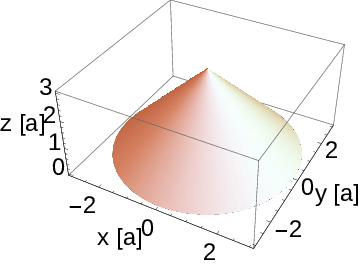
\includegraphics[width=0.8\linewidth]{cone.png}}
  \caption{
  Ytan $S_1$ uppritad. \label{fig:cone}
  }
\end{figure}
%\clearpage % flush figures fig:cone


\begin{itemize}
\item Undersök fältet $\vec{F}$. Singulariteter? Beräkna $\nabla \cdot \vec{F}$.
\end{itemize}

\noindent
Ska man använda Gauss sats så är det viktigt att man behandlar singulära delar av fältet korrekt, dvs identifiera \emph{källtermer} som är inneslutna innanför ytan. När man separerat de singulära delarna av fältet så kan man sen beräkna divergensen och utföra volymsintegralen. Vi skriver fältet $\vec{F}$ som två olika fält 
\begin{equation}
\vec{F}=\vec{F_1}+\vec{F_2}
\end{equation}
där 
\begin{align}
\vec{F_1}&= F_0 \frac{a^2}{(x^2+y^2+z^2)^{3/2}} \left( x,y,z \right ) = F_0 a^2 \frac{\hat{r}}{r^2}\\
\vec{F_2}&= F_0 \frac{z}{a}\hat{z}
\end{align}
För att skriva om fältet $\vec{F}_1$ till sfäriska kordinater har vi använt oss av att
\begin{align}
x\hat{x}+y\hat{y}+z\hat{z} = r\hat{r}\\
\sqrt{x^2+y^2+z^2}=r
\end{align}
Vi känner nu igen fältet $\vec{F}_1$ som fältet från en punktkälla i origo. Styrkan hos punktkällan är $4\pi F_0 a^2$. 

Fältet $\vec{F}_2$ motsvarar en rymdkälla med konstant källtäthet
\begin{equation}
\nabla \cdot \vec{F_2} = F_0 \partial_z \frac{z}{a} = \frac{F_0}{a}.
\end{equation}

\begin{itemize}
\item Slut ytan $S$. Undvik singulariteter inuti den inneslutna volymen.
\end{itemize}

\noindent
Gauss sats lyder 
\begin{equation}
\int_{S}\ \vec{F} \cdot d\vec{S} = \int_{V}\ \nabla \cdot \vec{F} dV
\end{equation} 
och det är viktigt att tänka på att $S=\partial V$, dvs ytan $S$ är randen till volymen $V$. Det betyder att $S$ måste vara en sluten yta (hur kan den annars vara randen till en volym?). Det betyder att för att kunna använda Gauss sats för denna uppgiften måste vi sluta konen. Det mest uppenbara sättet att sluta ytan är att lägga till en bottenplatta till konen. \footnote{Vi kan såklart sluta yan med något annat än en bottenplatta om vi vill. Tex kunde vi ta en halsvsfär och Gauss sats fungerar. Men för att det ska vara lönt att använda Gauss sats är det viktigt att den ytan vi lägger till är enklare att integrera över än originalytan.}

Bottenplattan motsvarar alltså cirkeln som konen ligger på i $x,y$ planet. Vi kallar denna ytan $S_2$ och skriver den som $S_2:\ x^2+y^2\leq (3a)^2$. 

Vi har dock ett litet problem nu: Punktkällan ligger mitt i bottenplattan, dvs på ytan. Hur ska man tänka nu? Vi kommer att illustrera \emph{tre} olika sätt att hantera denna punktkälla. 
\begin{enumerate}
\item Slut istället ytan på ett annat sätt så att punktkällan hamnar helt utanför.

\item Slut istället ytan på ett annat sätt så att punktkällan hamnar helt innanför.

\item Beräkna bidraget från punktkällan genom att räkna ut rymdvinkeln som konen upptar.
\end{enumerate}

\noindent
Alla tre metoderna kommer givetvis att ge samma svar. 

För att följa alt. 1 inför vi en halvsfär upp i det övre halvplanet med centrum i origo. Halvsfärens radie kallar vi $\epsilon$ och låter denna vara liten så att halvsfärens yta inte skär konens mantelyta. Denna nya yta kallar vi $S^+_\epsilon$. Tillsammans med $S_1$ och den modifierade bottenplattan $S_{2-\epsilon}$ bildas en sluten yta som \emph{inte} kommer att innesluta punktkällan i volymen. 

För att följa alt. 2 så sluter vi t.ex. ytan med en halvsfär ned i det nedre halvplanet med centrum i origo. Här kan vi låta radien vara lika med $3a$ så att vi direkt får en sluten yta av $S_1 + S^-_{3a}$ som omsluter punktkällan, där $S^-_{3a}$ är den införda halvsfärens yta.

För att följa alt. 3 handlar det bara om att beräkna hur stor rymdvinkel som konen upptar sedd från punktkällan. Se mer nedan.

\begin{itemize}
\item Teckna Gauss sats och beräkna integralen.
\end{itemize}

\noindent
Vi börjar med det oproblematiska bidraget från $\vec{F}_2$ med den sökta ytintegralen
\begin{equation}
I_2 \equiv \int_{S_1} \vec{F}_2 \cdot d\vec{S}
\end{equation}

Vi använder den slutna ytan $S_1+S_2$ som vi kan använda i Gauss sats
\begin{equation}
\int_{S_1+S_2} \vec{F}_2 \cdot d\vec{S} = \int_V \nabla \cdot \vec{F}_2 dV 
\end{equation}

Vi bollar över integralen över $S_2$ till andra sidan av likheten och får
\begin{equation}
\label{eq:GaussTot}
\int_{S_1} \vec{F}_2 \cdot d\vec{S} = \int_V \nabla \cdot \vec{F}_2 dV - \int_{S_2} \vec{F}_2 \cdot d\vec{S}
\end{equation}
där den ytintgral som uppgiften ber oss beräkna nu står i vänsterledet. Vi ser att det var viktigt att sluta ytan då vi nu har en extra term att dra bort från värdet av volymsintegralen. Nyttan med Gauss sats är som störst när divergensen är simpel och normalytintegralen över bottenplattan (eller vilken annan del man slutit sin yta med) är simpel.

Divergensen för $\vec{F}_2$ räknade vi ut ovan och vi får
\begin{equation}
\int_V \nabla \cdot \vec{F_2} dV = \frac{F_0}{a} \int_V dV = F_0 \pi (3a)^2
\end{equation}
där vi i det sista steget använt att volymen av en kon är $V=\pi r^2 h/3$ där $r$ är basradien och $h$ är höjden. 

Vi behöver nu ytintegralen över bottenlattan kvar enligt ekv. (\ref{eq:GaussTot}). Det är viktigt att notera att bottenplattans normalvektor pekar ut från den inneslutna volymen, dvs nedåt. Vi ska alltså beräkna 
\begin{equation}
\int_{S_2} \vec{F_2} \cdot d\vec{S} = -\int_{S_2} \vec{F_2} \cdot \hat{z} dS= -\int_{S_2} F_0\frac{z}{a}\hat{z} \cdot \hat{z} dS
\end{equation}
eftersom $z=0$ på $S_2$ så integralen över $\vec{F}_2$ på bottenplattan är noll. Vi har alltså att
\begin{equation}
I_2 = F_0 \pi (3a)^2
\end{equation}

Återstår integralen över $\vec{F}_1$. Enligt alt. 1 blir
\begin{equation}
\label{eq:GaussTot2}
I_1 = \int_{S_1} \vec{F}_1 \cdot d\vec{S} = \int_{V_1} \nabla \cdot \vec{F}_1 dV - \int_{S_{2-\epsilon}} \vec{F}_1 \cdot d\vec{S} - \int_{S^+_{\epsilon}} \vec{F}_1 \cdot d\vec{S}.
\end{equation}
Volymsintegralen görs här över en volym som inte inkluderar punktkällan. Den blir därför noll (divergensen $\nabla \cdot \vec{F}_1=0$ i hela denna volym). Ytintegralen över bottenplattan $S_{2-\epsilon}$ blir också noll eftersom fältets riktning $\hat{r}$ är vinkelrät mot ytans normalriktning. På denna yta ligger ju $\hat{r}$ alltid i $xy$ planet. Slutligen har vi integralen över halvsfären. Normalen måste här vara riktad i negativ $\hat{r}$-led för att peka ut från volymen
\begin{equation}
\int_{S^+_{\epsilon}} \vec{F_1} \cdot d\vec{S} = \int_{S^+_{\epsilon}} F_0 a^2 \frac{\hat{r}}{\epsilon^2} \cdot (-\hat{r}) \epsilon^2 \sin\theta \mbox{d}\theta \mbox{d}\phi= -F_0 a^2 2\pi 
\end{equation}
Slutligen får vi alltså $I_1 = 0 - 0 - (-F_0 a^2 2\pi ) = F_0 a^2 2\pi$.

Med alt. 2 har vi att
\begin{equation}
\label{eq:GaussTot3}
I_1 = \int_{S_1} \vec{F}_1 \cdot d\vec{S} = \int_{V_2} \nabla \cdot \vec{F}_1 dV - \int_{S^-_{3a}} \vec{F}_1 \cdot d\vec{S}.
\end{equation}
Nu kommer volymen $V_2$ att innesluta punktkällan och bidraget från denna term blir lika med punktkällans styrka: $F_0 a^2 4\pi$. Ytintegralen över $S^-_{3a}$ göra på precis samma sätt som ovan, men vi skall nu notera att normalriktningen pekar i positiv $\hat{r}$-led för att peka ut från volymen. Bidraget blir $F_0 a^2 2\pi$. Slutligen ger alltså denna metod att $I_1 = F_0 a^2 4\pi - F_0 a^2 2\pi = F_0 a^2 2\pi$, precis som alt. 1 ovan.

Enligt alt. 3 hade vi direkt kunnat räkna ut ytintegralen över konens mantelyta med Cederwall ekv. 6.7. Sett från punktkällan i origo upptar konens mantelyta en rymdvinkel $2\pi$. Det totala bidraget blir därför $(2\pi)/(4\pi) = 1/2$ av punktkällans styrka. Dvs vi får $I_1 = (F_0 a^2 4\pi)/2 = F_0 a^2 2\pi$. Givetvis samma resultat som med alt. 1 och 2.

Nu kombinerar vi ihop våra delresultat
\begin{equation}
\int_{S_1} \vec{F} \cdot d\vec{S} = I_1 + I_2 = F_0 a^2 2\pi + F_0 \pi (3a)^2 = F_0 \pi 11 a^2
\end{equation}

\begin{itemize}
\item Har normalen rätt riktning?
\end{itemize}

\noindent
Kontrollera gärna en gång till att ytnormalerna i de ytintegraler som ger nollskilda bidrag har rätt bidrag. Detta gäller i synnerhet de två halvsfärer som vi införde för att räkna ut $I_1$ enligt alt. 1 och alt. 2.

Svaret på uppgiften är alltså $11\pi F_0 a^2$.

Kontrollera också dimensionen på svaret. Vårt fält har dimensionen $[F_0]$ och ytintegralen skall därför ha dimensionen $[F_0]$*area, vilket verkar stämma.

% --- end solution of exercise ---

% Closing remarks for this Exercise

\paragraph{Remarks.}
Uppgiften illustrerar olika sätt att hantera en singularitet som hamnar på randen till en volym.

Det är värt att notera att den här uppgiften innehåller ett icke-standard moment som utgörs av att punktkällan ligger på den bottenyta som är naturlig att sluta ytan med. 

Notera att vi i slutändan fick precis halva styrkan 
av punktkällan som bidrag oavsett vilken metod vi använde för att hantera den. Det betyder att det kanske enklaste sättet att se detta på är att punktkällan strålar 
halva sitt bidrag in mot konen $S_1$ i detta fallet, dvs man tänker som i 
metod 3.


\end{doconceexercise}
% --- end exercise ---


% ------------------- end of main content ---------------

\end{document}

